% DPF 09 talk on strangeness in nucleon

\documentclass[10pt]{beamer}
\usepackage{amsmath}
\usepackage{mathtools}
%\documentclass[12pt]{beamerthemeSam.sty}
\usepackage{epsf}
%\usepackage{pstricks}
%\usepackage[orientation=portrait,size=A4]{beamerposter}
\geometry{paperwidth=160mm,paperheight=120mm}
%DT favorite definitions
\def\LL{\left\langle}	% left angle bracket
\def\RR{\right\rangle}	% right angle bracket
\def\LP{\left(}		% left parenthesis
\def\RP{\right)}	% right parenthesis
\def\LB{\left\{}	% left curly bracket
\def\RB{\right\}}	% right curly bracket
\def\PAR#1#2{ {{\partial #1}\over{\partial #2}} }
\def\PARTWO#1#2{ {{\partial^2 #1}\over{\partial #2}^2} }
\def\PARTWOMIX#1#2#3{ {{\partial^2 #1}\over{\partial #2 \partial #3}} }

\def\rightpartial{{\overrightarrow\partial}}
\def\leftpartial{{\overleftarrow\partial}}
\def\diffpartial{\buildrel\leftrightarrow\over\partial}

\def\BI{\begin{itemize}}
\def\EI{\end{itemize}}
\def\BE{\begin{displaymath}}
\def\EE{\end{displaymath}}
\def\BEA{\begin{eqnarray*}}
\def\EEA{\end{eqnarray*}}
\def\BNEA{\begin{eqnarray}}
\def\ENEA{\end{eqnarray}}
\def\EL{\nonumber\\}


\newcommand{\map}[1]{\frame{\frametitle{\textbf{Course map}}
\centerline{\includegraphics[height=0.86\paperheight]{../../map/#1.png}}}}
\newcommand{\wmap}[1]{\frame{\frametitle{\textbf{Course map}}
\centerline{\includegraphics[width=0.96\paperwidth]{../../map/#1.png}}}}

\newcommand{\etal}{{\it et al.}}
\newcommand{\gbeta}{6/g^2}
\newcommand{\la}[1]{\label{#1}}
\newcommand{\ie}{{\em i.e.\ }}
\newcommand{\eg}{{\em e.\,g.\ }}
\newcommand{\cf}{cf.\ }
\newcommand{\etc}{etc.\ }
\newcommand{\atantwo}{{\rm atan2}}
\newcommand{\Tr}{{\rm Tr}}
\newcommand{\dt}{\Delta t}
\newcommand{\op}{{\cal O}}
\newcommand{\msbar}{{\overline{\rm MS}}}
\def\chpt{\raise0.4ex\hbox{$\chi$}PT}
\def\schpt{S\raise0.4ex\hbox{$\chi$}PT}
\def\MeV{{\rm Me\!V}}
\def\GeV{{\rm Ge\!V}}

%AB: my color definitions
%\definecolor{mygarnet}{rgb}{0.445,0.184,0.215}
%\definecolor{mygold}{rgb}{0.848,0.848,0.098}
%\definecolor{myg2g}{rgb}{0.647,0.316,0.157}
\definecolor{abtitlecolor}{rgb}{0.0,0.255,0.494}
\definecolor{absecondarycolor}{rgb}{0.0,0.416,0.804}
\definecolor{abprimarycolor}{rgb}{1.0,0.686,0.0}
\definecolor{Red}           {cmyk}{0,1,1,0}
\definecolor{Grey}           {cmyk}{.7,.7,.7,0}
\definecolor{Blue}          {cmyk}{1,1,0,0}
\definecolor{Green}         {cmyk}{1,0,1,0}
\definecolor{Brown}         {cmyk}{0,0.81,1,0.60}
\definecolor{Black}         {cmyk}{0,0,0,1}

\usetheme{Madrid}


%AB: redefinition of beamer colors
%\setbeamercolor{palette tertiary}{fg=white,bg=mygarnet}
%\setbeamercolor{palette secondary}{fg=white,bg=myg2g}
%\setbeamercolor{palette primary}{fg=black,bg=mygold}
\setbeamercolor{title}{fg=abtitlecolor}
\setbeamercolor{frametitle}{fg=abtitlecolor}
\setbeamercolor{palette tertiary}{fg=white,bg=abtitlecolor}
\setbeamercolor{palette secondary}{fg=white,bg=absecondarycolor}
\setbeamercolor{palette primary}{fg=black,bg=abprimarycolor}
\setbeamercolor{structure}{fg=abtitlecolor}

\setbeamerfont{section in toc}{series=\bfseries}

%AB: remove navigation icons
\beamertemplatenavigationsymbolsempty
\title[Friction (etc.)]{
  \textbf {Friction (and sundry)}\\
%\centerline{}
%\centering
%\vspace{-0.0in}
%\includegraphics[width=0.3\textwidth]{propvalues_0093.pdf}
%\vspace{-0.3in}\\
%\label{intrograph}
}

\author[W. Freeman] {Physics 211\\Syracuse University, Physics 211 Spring 2015\\Walter Freeman}

\date{\today}

\begin{document}

\frame{\titlepage}

\frame{\frametitle{\textbf{Announcements}}
\BI
\Large
\item{Homework 4 should be posted today}
\item{Another {\it Mastering Physics} assignment should be posted today (due Tuesday before class)}
\item{Another {\it Mastering Physics} assignment should be posted today (due next Thursday before class)}
\item{Read Chapter 8 for Thursday (don't worry if you don't understand everything -- {\it yet!})}
  \pause
\item{Late MP submissions accepted for the previous MP assignment until end of day (I'll fix it)}
\EI

}

\frame{\frametitle{\textbf{Ask a Physicist: Special relativity}}
``Suppose for a moment that the universe was infinitely large with nearly an infinite amount of mass. Now, suppose all that mass was put into two objects at an incredibly far distance away. Now, due to gravity these objects begin to accelerate towards each other at a rate that would resemble earth's gravity for trillions of years. Is the maximum speed these objects will reach be the speed of light? If so, does this mean that gravity is relative to the speed of light?''
}

\frame{\frametitle{\textbf{Ask a Physicist: Special relativity}}
``Suppose that an 1N object is subjected to a constant force for ten billions years. What happens to its speed?'' 

\pause

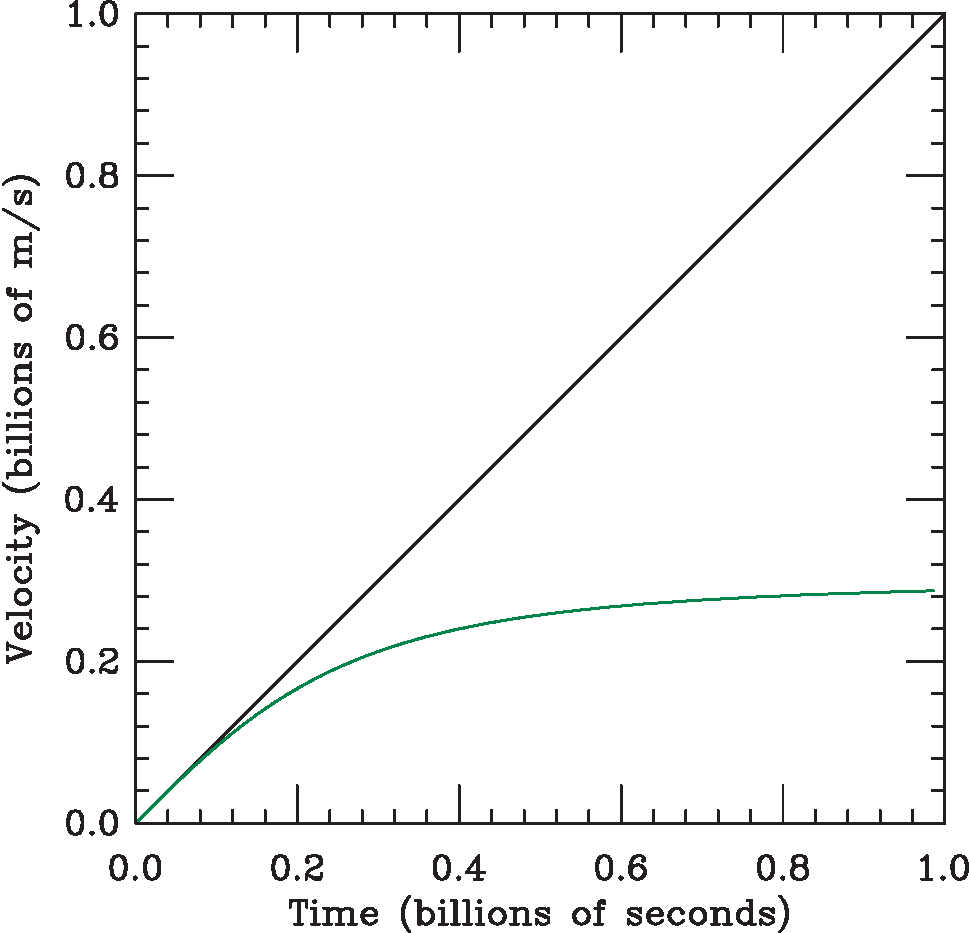
\includegraphics[width=0.5\textwidth]{rel-1-crop.pdf}
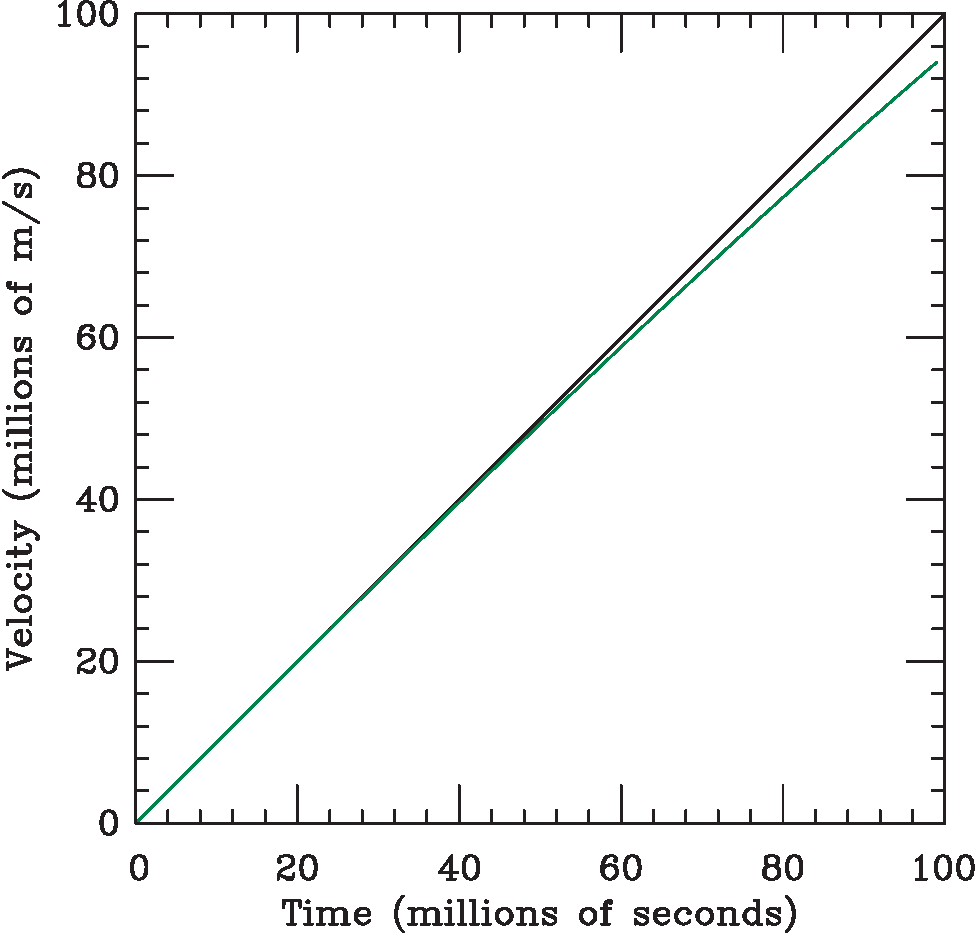
\includegraphics[width=0.5\textwidth]{rel-2-crop.pdf}

}


\frame{\frametitle{\textbf{Homework review: Problem 1}}
  \BI
\item{Only two forces: normal force of the ground on her feet, and her weight}
\EI

\Large
\centerline{$\sum F = ma$}
\centerline{$F_N - mg = ma$}
\centerline{$F_N = mg + ma$}
}

\frame{\frametitle{\textbf{Homework review: Problem 6}}
  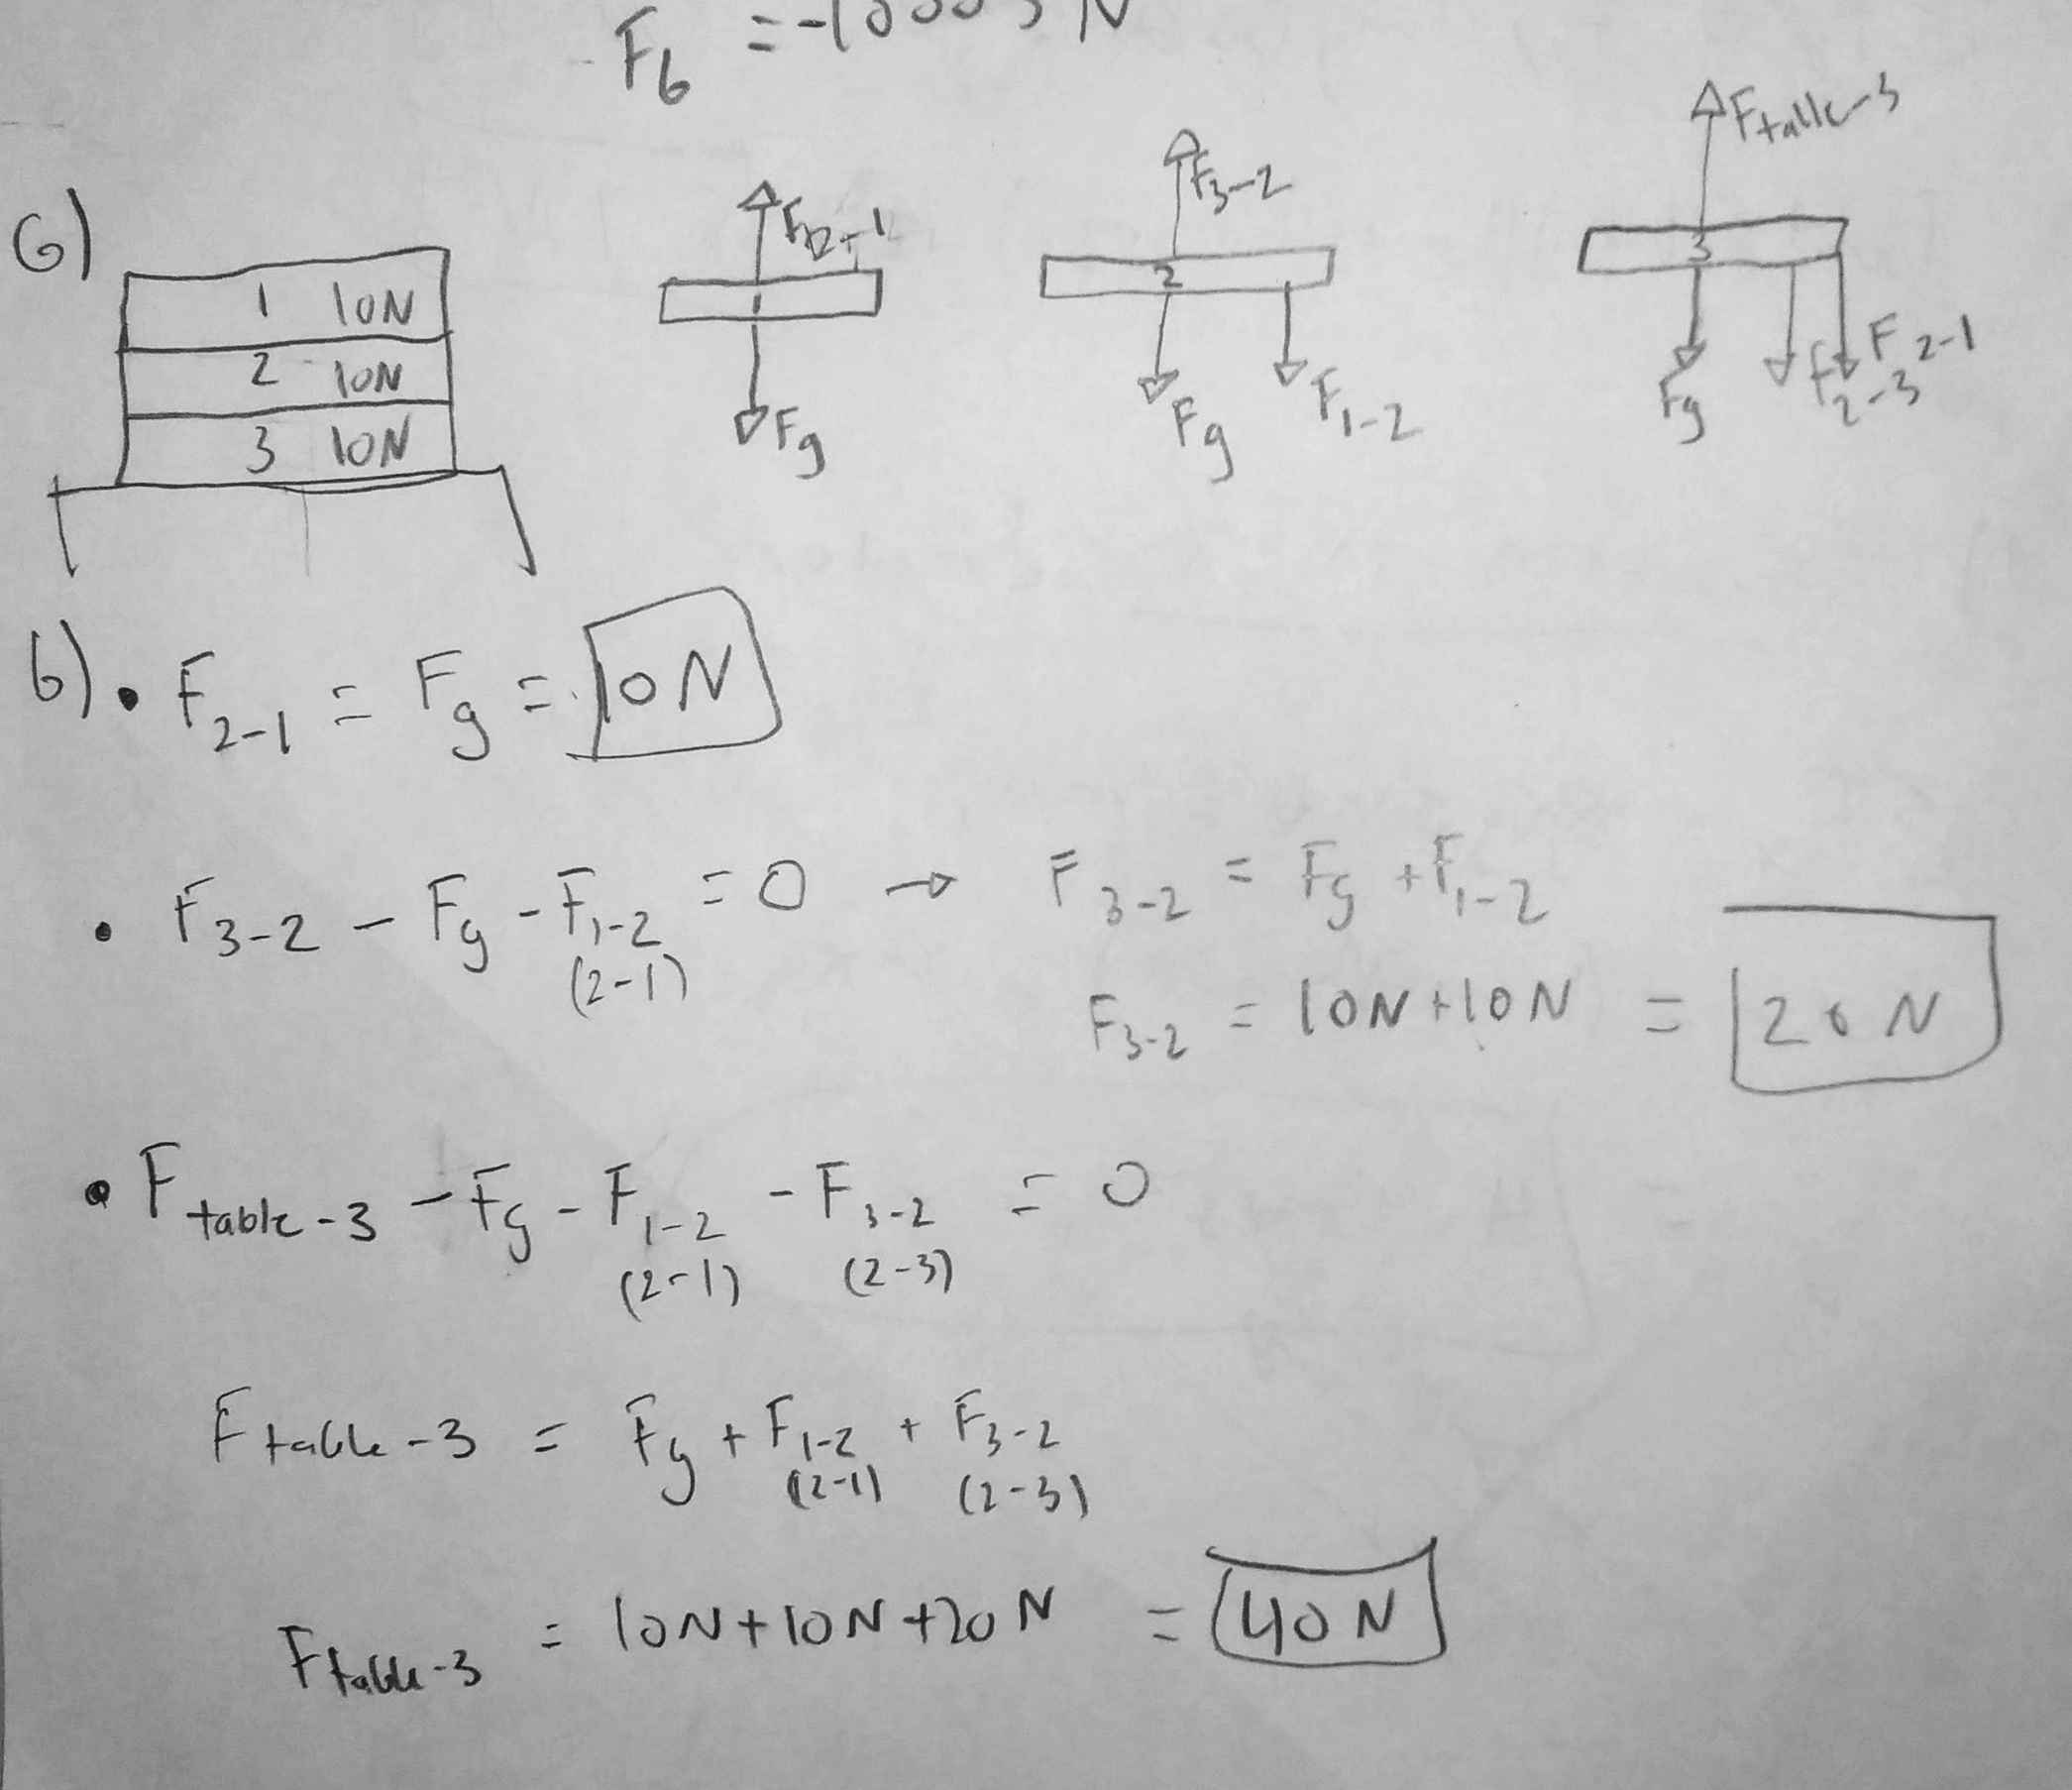
\includegraphics[width=0.6\textwidth]{problem-6.jpg}
}
  

\frame{\frametitle{\textbf{A new force: Friction}}
  \large
  \BI
\item{Friction: stops two surfaces from sliding past each other}
\item{Can either make things move or make things stop; opposes {\it relative} motion}
\item{Two types:}
\BI
\item{Static friction: keeps two things that aren't sliding stuck together}
\item{Kinetic friction: opposes the relative motion of two things sliding}
\EI
\EI
}

\frame{\frametitle{\textbf{Coulomb's friction model}}
  \large
  \centerline{Friction is really complicated!}
  \BI
\item{Depends on details of surfaces, molecular forces, etc.}
\item{No way to create a completely accurate general principle}
  \EI

  \bigskip
  \bigskip

  \centerline{There are a few general principles, though:}
  \BI
\item{Friction is higher if the normal force is higher}
\item{Kinetic friction doesn't depend that much on the speed of travel}
  \EI
  
  \bigskip
  \bigskip
  
  \centerline{Simple model: often pretty close}
  \BI
\item{Friction depends on a property of the surfaces called the {\color{Red}coefficient of friction} $\mu$}
\item{Force of kinetic friction = $\mu_k F_N$}
\item{Max force of static friction = $\mu_s F_N$}
  \EI
}

\frame{\frametitle{\textbf{Coefficients of friction}}

  \centerline { 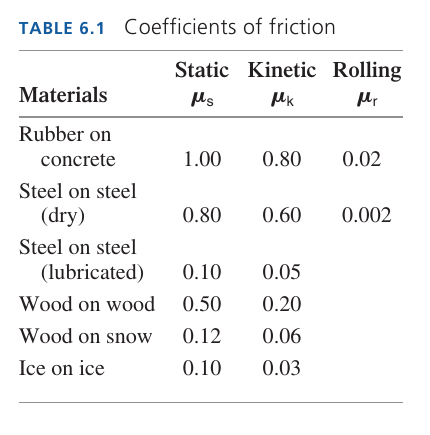
\includegraphics[width=0.5\textwidth]{mu-table.png}}
}

\frame{\frametitle{\textbf{A discussion of rolling}}
  \large
``Rolling without slipping'':
  \BI
\item{Neither static friction nor kinetic friction opposes rolling}
\item{Point of contact doesn't slide (wheels work well!)}
\item{Some residual loss of energy from ``rolling friction'' (flexing of the wheel)}
\item{Static friction required to {\it keep} an object rolling without slipping sometimes}
  \EI
}

\frame{\frametitle{\textbf{Problem solving: friction}}
\Large
\centerline{Friction links the $x$ and $y$ directions:}

\large
\BI
\item{Friction acts parallel to the surface (appears in $\sum F_x = m a_x$}
\item{Friction {\it depends} on the normal force, perpendicular to the surface (appears in $\sum F_y = m a_y$}
  \EI

  \centerline{This doesn't change how you should solve problems!}

  \BI
\item{{\color{Red}Accounting:} Draw force diagrams for every object (friction and normal force appear)}
  \pause
\item{{\color{Red}Physics:} Write down $\sum F = ma$ in each dimension, for each object (with $F_N$ and $\mu F_N$}
  \pause
\item{{\color{Red}Math:} Put in the stuff you know, solve for the stuff you don't; find $F_N$, substitute...}
  \pause
\item{{\color{Red}Kinematics:} Connect acceleration to motion}
  \EI
}



  

  \frame{\frametitle{\textbf{Sample questions}}
    \Large

    A cart slides down a track elevated at angle $\theta$ with $\mu_k$ known; what is its acceleration?
  } 

  \frame{\frametitle{\textbf{Sample questions}}
    \Large

    Two masses of 20 and 40 kg hang from a massless pulley on either side. How do they move?
  } 

  \frame{\frametitle{\textbf{Sample questions}}
    \Large

    Two masses of $m_1$ and $m_2$ kg hang from a massless pulley on either side. How do they move?
  } 

  \frame{\frametitle{\textbf{Sample questions}}
    \Large
  A cart with mass $m$ on a track is connected by a rope to a hanging weight of mass $M$. The coefficient of friction is $\mu$. What is the acceleration of both objects?

  } 

  \end{document}

